% =========================================================
% DIAGRAMA: Estructura paquete BLE NUS (Nordic UART Service)
% Archivo imagen: Ilustraciones/ble_nus_packet.png
%
% QUÉ DIBUJAR EN DRAW.IO:
%   Pila de capas BLE de arriba a abajo:
%
%   ┌─────────────────────────────────────────────────┐
%   │  Aplicación: JSON payload                        │
%   │  {"cmd":"snapshot"}  /  {"pid":12,"value":1724} │
%   ├─────────────────────────────────────────────────┤
%   │  ATT (Attribute Protocol)                        │
%   │  Handle: 0x000E (RX char) / 0x000B (TX char)   │
%   ├─────────────────────────────────────────────────┤
%   │  GATT Characteristic                            │
%   │  RX: 6E400002-... (Write / Write-No-Response)   │
%   │  TX: 6E400003-... (Notify)                      │
%   ├─────────────────────────────────────────────────┤
%   │  GATT Service: NUS                              │
%   │  UUID: 6E400001-B5A3-F393-E0A9-E50E24DCCA9E    │
%   ├─────────────────────────────────────────────────┤
%   │  L2CAP / LE-U logical link                      │
%   │  MTU negociado: 240 bytes                       │
%   ├─────────────────────────────────────────────────┤
%   │  BLE Link Layer / Radio 2.4 GHz                 │
%   └─────────────────────────────────────────────────┘
%
%   - Cada capa = rectángulo con color distinto
%   - Flecha bidireccional a la derecha indicando dirección: App→RPi / RPi→App
%   - Nota: "Max payload: 240 - 3 bytes ATT overhead = 237 bytes"
%   - Título: "Pila de protocolos BLE NUS"
% =========================================================

\centering
% TODO draw.io: pila de capas BLE NUS (App JSON → ATT → GATT RX/TX → L2CAP → Radio) y exportar como ble_nus_packet.png
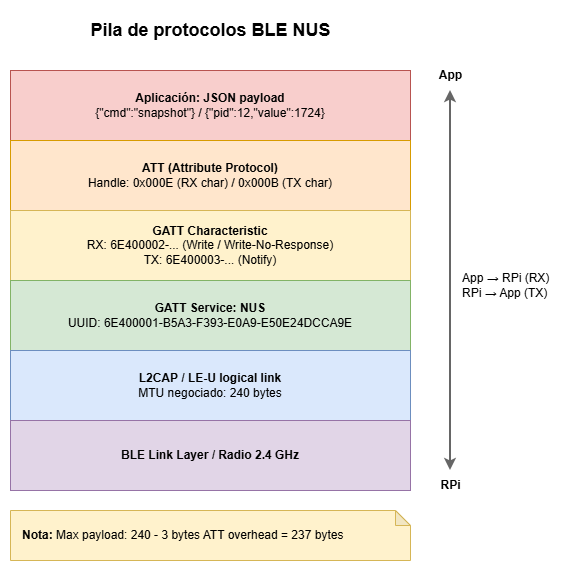
\includegraphics[width=0.5\textwidth]{Ilustraciones/BLE_layers.png}
